%% template.tex
%% from
%% bare_conf.tex
%% V1.4b
%% 2015/08/26
%% by Michael Shell
%% See:
%% http://www.michaelshell.org/
%% for current contact information.
%%
%% This is a skeleton file demonstrating the use of IEEEtran.cls
%% (requires IEEEtran.cls version 1.8b or later) with an IEEE
%% conference paper.
%%
%% Support sites:
%% http://www.michaelshell.org/tex/ieeetran/
%% http://www.ctan.org/pkg/ieeetran
%% and
%% http://www.ieee.org/

%%*************************************************************************
%% Legal Notice:
%% This code is offered as-is without any warranty either expressed or
%% implied; without even the implied warranty of MERCHANTABILITY or
%% FITNESS FOR A PARTICULAR PURPOSE!
%% User assumes all risk.
%% In no event shall the IEEE or any contributor to this code be liable for
%% any damages or losses, including, but not limited to, incidental,
%% consequential, or any other damages, resulting from the use or misuse
%% of any information contained here.
%%
%% All comments are the opinions of their respective authors and are not
%% necessarily endorsed by the IEEE.
%%
%% This work is distributed under the LaTeX Project Public License (LPPL)
%% ( http://www.latex-project.org/ ) version 1.3, and may be freely used,
%% distributed and modified. A copy of the LPPL, version 1.3, is included
%% in the base LaTeX documentation of all distributions of LaTeX released
%% 2003/12/01 or later.
%% Retain all contribution notices and credits.
%% ** Modified files should be clearly indicated as such, including  **
%% ** renaming them and changing author support contact information. **
%%*************************************************************************


% *** Authors should verify (and, if needed, correct) their LaTeX system  ***
% *** with the testflow diagnostic prior to trusting their LaTeX platform ***
% *** with production work. The IEEE's font choices and paper sizes can   ***
% *** trigger bugs that do not appear when using other class files.       ***                          ***
% The testflow support page is at:
% http://www.michaelshell.org/tex/testflow/

\documentclass[conference,final,]{IEEEtran}
% Some Computer Society conferences also require the compsoc mode option,
% but others use the standard conference format.
%
% If IEEEtran.cls has not been installed into the LaTeX system files,
% manually specify the path to it like:
% \documentclass[conference]{../sty/IEEEtran}





% Some very useful LaTeX packages include:
% (uncomment the ones you want to load)


% *** MISC UTILITY PACKAGES ***
%
%\usepackage{ifpdf}
% Heiko Oberdiek's ifpdf.sty is very useful if you need conditional
% compilation based on whether the output is pdf or dvi.
% usage:
% \ifpdf
%   % pdf code
% \else
%   % dvi code
% \fi
% The latest version of ifpdf.sty can be obtained from:
% http://www.ctan.org/pkg/ifpdf
% Also, note that IEEEtran.cls V1.7 and later provides a builtin
% \ifCLASSINFOpdf conditional that works the same way.
% When switching from latex to pdflatex and vice-versa, the compiler may
% have to be run twice to clear warning/error messages.






% *** CITATION PACKAGES ***
%
%\usepackage{cite}
% cite.sty was written by Donald Arseneau
% V1.6 and later of IEEEtran pre-defines the format of the cite.sty package
% \cite{} output to follow that of the IEEE. Loading the cite package will
% result in citation numbers being automatically sorted and properly
% "compressed/ranged". e.g., [1], [9], [2], [7], [5], [6] without using
% cite.sty will become [1], [2], [5]--[7], [9] using cite.sty. cite.sty's
% \cite will automatically add leading space, if needed. Use cite.sty's
% noadjust option (cite.sty V3.8 and later) if you want to turn this off
% such as if a citation ever needs to be enclosed in parenthesis.
% cite.sty is already installed on most LaTeX systems. Be sure and use
% version 5.0 (2009-03-20) and later if using hyperref.sty.
% The latest version can be obtained at:
% http://www.ctan.org/pkg/cite
% The documentation is contained in the cite.sty file itself.






% *** GRAPHICS RELATED PACKAGES ***
%
\ifCLASSINFOpdf
  % \usepackage[pdftex]{graphicx}
  % declare the path(s) where your graphic files are
  % \graphicspath{{../pdf/}{../jpeg/}}
  % and their extensions so you won't have to specify these with
  % every instance of \includegraphics
  % \DeclareGraphicsExtensions{.pdf,.jpeg,.png}
\else
  % or other class option (dvipsone, dvipdf, if not using dvips). graphicx
  % will default to the driver specified in the system graphics.cfg if no
  % driver is specified.
  % \usepackage[dvips]{graphicx}
  % declare the path(s) where your graphic files are
  % \graphicspath{{../eps/}}
  % and their extensions so you won't have to specify these with
  % every instance of \includegraphics
  % \DeclareGraphicsExtensions{.eps}
\fi
% graphicx was written by David Carlisle and Sebastian Rahtz. It is
% required if you want graphics, photos, etc. graphicx.sty is already
% installed on most LaTeX systems. The latest version and documentation
% can be obtained at:
% http://www.ctan.org/pkg/graphicx
% Another good source of documentation is "Using Imported Graphics in
% LaTeX2e" by Keith Reckdahl which can be found at:
% http://www.ctan.org/pkg/epslatex
%
% latex, and pdflatex in dvi mode, support graphics in encapsulated
% postscript (.eps) format. pdflatex in pdf mode supports graphics
% in .pdf, .jpeg, .png and .mps (metapost) formats. Users should ensure
% that all non-photo figures use a vector format (.eps, .pdf, .mps) and
% not a bitmapped formats (.jpeg, .png). The IEEE frowns on bitmapped formats
% which can result in "jaggedy"/blurry rendering of lines and letters as
% well as large increases in file sizes.
%
% You can find documentation about the pdfTeX application at:
% http://www.tug.org/applications/pdftex

\usepackage{graphicx}

% *** MATH PACKAGES ***
%
\usepackage{amsmath}
\interdisplaylinepenalty=2500
%\usepackage{amsmath}
% A popular package from the American Mathematical Society that provides
% many useful and powerful commands for dealing with mathematics.
%
% Note that the amsmath package sets \interdisplaylinepenalty to 10000
% thus preventing page breaks from occurring within multiline equations. Use:
%\interdisplaylinepenalty=2500
% after loading amsmath to restore such page breaks as IEEEtran.cls normally
% does. amsmath.sty is already installed on most LaTeX systems. The latest
% version and documentation can be obtained at:
% http://www.ctan.org/pkg/amsmath





% *** SPECIALIZED LIST PACKAGES ***
%
%\usepackage{algorithmic}
% algorithmic.sty was written by Peter Williams and Rogerio Brito.
% This package provides an algorithmic environment fo describing algorithms.
% You can use the algorithmic environment in-text or within a figure
% environment to provide for a floating algorithm. Do NOT use the algorithm
% floating environment provided by algorithm.sty (by the same authors) or
% algorithm2e.sty (by Christophe Fiorio) as the IEEE does not use dedicated
% algorithm float types and packages that provide these will not provide
% correct IEEE style captions. The latest version and documentation of
% algorithmic.sty can be obtained at:
% http://www.ctan.org/pkg/algorithms
% Also of interest may be the (relatively newer and more customizable)
% algorithmicx.sty package by Szasz Janos:
% http://www.ctan.org/pkg/algorithmicx




% *** ALIGNMENT PACKAGES ***
%
%\usepackage{array}
% Frank Mittelbach's and David Carlisle's array.sty patches and improves
% the standard LaTeX2e array and tabular environments to provide better
% appearance and additional user controls. As the default LaTeX2e table
% generation code is lacking to the point of almost being broken with
% respect to the quality of the end results, all users are strongly
% advised to use an enhanced (at the very least that provided by array.sty)
% set of table tools. array.sty is already installed on most systems. The
% latest version and documentation can be obtained at:
% http://www.ctan.org/pkg/array


% IEEEtran contains the IEEEeqnarray family of commands that can be used to
% generate multiline equations as well as matrices, tables, etc., of high
% quality.




% *** SUBFIGURE PACKAGES ***
%\ifCLASSOPTIONcompsoc
%  \usepackage[caption=false,font=normalsize,labelfont=sf,textfont=sf]{subfig}
%\else
%  \usepackage[caption=false,font=footnotesize]{subfig}
%\fi
% subfig.sty, written by Steven Douglas Cochran, is the modern replacement
% for subfigure.sty, the latter of which is no longer maintained and is
% incompatible with some LaTeX packages including fixltx2e. However,
% subfig.sty requires and automatically loads Axel Sommerfeldt's caption.sty
% which will override IEEEtran.cls' handling of captions and this will result
% in non-IEEE style figure/table captions. To prevent this problem, be sure
% and invoke subfig.sty's "caption=false" package option (available since
% subfig.sty version 1.3, 2005/06/28) as this is will preserve IEEEtran.cls
% handling of captions.
% Note that the Computer Society format requires a larger sans serif font
% than the serif footnote size font used in traditional IEEE formatting
% and thus the need to invoke different subfig.sty package options depending
% on whether compsoc mode has been enabled.
%
% The latest version and documentation of subfig.sty can be obtained at:
% http://www.ctan.org/pkg/subfig




% *** FLOAT PACKAGES ***
%

%\usepackage{fixltx2e}
% fixltx2e, the successor to the earlier fix2col.sty, was written by
% Frank Mittelbach and David Carlisle. This package corrects a few problems
% in the LaTeX2e kernel, the most notable of which is that in current
% LaTeX2e releases, the ordering of single and double column floats is not
% guaranteed to be preserved. Thus, an unpatched LaTeX2e can allow a
% single column figure to be placed prior to an earlier double column
% figure.
% Be aware that LaTeX2e kernels dated 2015 and later have fixltx2e.sty's
% corrections already built into the system in which case a warning will
% be issued if an attempt is made to load fixltx2e.sty as it is no longer
% needed.
% The latest version and documentation can be found at:
% http://www.ctan.org/pkg/fixltx2e


%\usepackage{stfloats}
% stfloats.sty was written by Sigitas Tolusis. This package gives LaTeX2e
% the ability to do double column floats at the bottom of the page as well
% as the top. (e.g., "\begin{figure*}[!b]" is not normally possible in
% LaTeX2e). It also provides a command:
%\fnbelowfloat
% to enable the placement of footnotes below bottom floats (the standard
% LaTeX2e kernel puts them above bottom floats). This is an invasive package
% which rewrites many portions of the LaTeX2e float routines. It may not work
% with other packages that modify the LaTeX2e float routines. The latest
% version and documentation can be obtained at:
% http://www.ctan.org/pkg/stfloats
% Do not use the stfloats baselinefloat ability as the IEEE does not allow
% \baselineskip to stretch. Authors submitting work to the IEEE should note
% that the IEEE rarely uses double column equations and that authors should try
% to avoid such use. Do not be tempted to use the cuted.sty or midfloat.sty
% packages (also by Sigitas Tolusis) as the IEEE does not format its papers in
% such ways.
% Do not attempt to use stfloats with fixltx2e as they are incompatible.
% Instead, use Morten Hogholm'a dblfloatfix which combines the features
% of both fixltx2e and stfloats:
%
% \usepackage{dblfloatfix}
% The latest version can be found at:
% http://www.ctan.org/pkg/dblfloatfix




% *** PDF, URL AND HYPERLINK PACKAGES ***
%
%\usepackage{url}
% url.sty was written by Donald Arseneau. It provides better support for
% handling and breaking URLs. url.sty is already installed on most LaTeX
% systems. The latest version and documentation can be obtained at:
% http://www.ctan.org/pkg/url
% Basically, \url{my_url_here}.




% *** Do not adjust lengths that control margins, column widths, etc. ***
% *** Do not use packages that alter fonts (such as pslatex).         ***
% There should be no need to do such things with IEEEtran.cls V1.6 and later.
% (Unless specifically asked to do so by the journal or conference you plan
% to submit to, of course. )



%% BEGIN MY ADDITIONS %%


\usepackage[unicode=true]{hyperref}

\hypersetup{
            pdftitle={Évolution de la diversité de Lépidoptères selon un gradient spatial au Québec},
            pdfkeywords={Lépidoptère, iNaturalist, Science
citoyenne, Zones climatiques, Changements climatiques},
            pdfborder={0 0 0},
            breaklinks=true}
\urlstyle{same}  % don't use monospace font for urls

% Pandoc toggle for numbering sections (defaults to be off)
\setcounter{secnumdepth}{0}


% tightlist command for lists without linebreak
\providecommand{\tightlist}{%
  \setlength{\itemsep}{0pt}\setlength{\parskip}{0pt}}


% Pandoc citation processing
%From Pandoc 3.1.8
% definitions for citeproc citations
\NewDocumentCommand\citeproctext{}{}
\NewDocumentCommand\citeproc{mm}{%
  \begingroup\def\citeproctext{#2}\cite{#1}\endgroup}
\makeatletter
 % allow citations to break across lines
 \let\@cite@ofmt\@firstofone
 % avoid brackets around text for \cite:
 \def\@biblabel#1{}
 \def\@cite#1#2{{#1\if@tempswa , #2\fi}}
\makeatother
\newlength{\cslhangindent}
\setlength{\cslhangindent}{1.5em}
\newlength{\csllabelwidth}
\setlength{\csllabelwidth}{3em}
\newenvironment{CSLReferences}[2] % #1 hanging-indent, #2 entry-spacing
 {\begin{list}{}{%
  \setlength{\itemindent}{0pt}
  \setlength{\leftmargin}{0pt}
  \setlength{\parsep}{0pt}
  % turn on hanging indent if param 1 is 1
  \ifodd #1
   \setlength{\leftmargin}{\cslhangindent}
   \setlength{\itemindent}{-1\cslhangindent}
  \fi
  % set entry spacing
  \setlength{\itemsep}{#2\baselineskip}}}
 {\end{list}}
\usepackage{calc}
\newcommand{\CSLBlock}[1]{#1\hfill\break}
\newcommand{\CSLLeftMargin}[1]{\parbox[t]{\csllabelwidth}{#1}}
\newcommand{\CSLRightInline}[1]{\parbox[t]{\linewidth - \csllabelwidth}{#1}\break}
\newcommand{\CSLIndent}[1]{\hspace{\cslhangindent}#1}

\usepackage{float}

%% END MY ADDITIONS %%


\hyphenation{op-tical net-works semi-conduc-tor}

\begin{document}
%
% paper title
% Titles are generally capitalized except for words such as a, an, and, as,
% at, but, by, for, in, nor, of, on, or, the, to and up, which are usually
% not capitalized unless they are the first or last word of the title.
% Linebreaks \\ can be used within to get better formatting as desired.
% Do not put math or special symbols in the title.
\title{Évolution de la diversité de Lépidoptères selon un gradient
spatial au Québec}

% author names and affiliations
% use a multiple column layout for up to three different
% affiliations

\author{

%% ---- classic IEEETrans wide authors' list ----------------
\IEEEauthorblockN{
Laurent Fournelle-Grenier,Clovis Marion,Léane Plouffe,Mariève Trottier%%
}


%% ----------------------------------------------------------

%% ---- classic IEEETrans one column per institution --------
 %%
%% ----------------------------------------------------------





%% ---- one column per author, classic/default IEEETrans ----

%% ----------------------------------------------------------

}

% conference papers do not typically use \thanks and this command
% is locked out in conference mode. If really needed, such as for
% the acknowledgment of grants, issue a \IEEEoverridecommandlockouts
% after \documentclass

% for over three affiliations, or if they all won't fit within the width
% of the page, use this alternative format:
%
%\author{\IEEEauthorblockN{Michael Shell\IEEEauthorrefmark{1},
%Homer Simpson\IEEEauthorrefmark{2},
%James Kirk\IEEEauthorrefmark{3},
%Montgomery Scott\IEEEauthorrefmark{3} and
%Eldon Tyrell\IEEEauthorrefmark{4}}
%\IEEEauthorblockA{\IEEEauthorrefmark{1}School of Electrical and Computer Engineering\\
%Georgia Institute of Technology,
%Atlanta, Georgia 30332--0250\\ Email: see http://www.michaelshell.org/contact.html}
%\IEEEauthorblockA{\IEEEauthorrefmark{2}Twentieth Century Fox, Springfield, USA\\
%Email: homer@thesimpsons.com}
%\IEEEauthorblockA{\IEEEauthorrefmark{3}Starfleet Academy, San Francisco, California 96678-2391\\
%Telephone: (800) 555--1212, Fax: (888) 555--1212}
%\IEEEauthorblockA{\IEEEauthorrefmark{4}Tyrell Inc., 123 Replicant Street, Los Angeles, California 90210--4321}}




% use for special paper notices
%\IEEEspecialpapernotice{(Invited Paper)}




% make the title area
\maketitle

% As a general rule, do not put math, special symbols or citations
% in the abstract
\begin{abstract}
Dans un contexte de changements environnementaux rapides, les structures
des communautés d'insectes, dont les lépidoptères, subissent
d'importantes transformations. Cette étude s'appuie sur des données,
provenant en partie d'observations citoyennes, pour analyser la
distribution spatiale des lépidoptères au Québec. La richesse spécifique
est examinée selon la latitude et la longitude, afin de détecter des
tendances spatiales liées aux zones climatiques du territoire québécois.
\end{abstract}

% keywords
\begin{IEEEkeywords}
Lépidoptère; iNaturalist; Science citoyenne; Zones
climatiques; Changements climatiques
\end{IEEEkeywords}

% use for special paper notices



% make the title area
\maketitle

% no keywords

% For peer review papers, you can put extra information on the cover
% page as needed:
% \ifCLASSOPTIONpeerreview
% \begin{center} \bfseries EDICS Category: 3-BBND \end{center}
% \fi
%
% For peerreview papers, this IEEEtran command inserts a page break and
% creates the second title. It will be ignored for other modes.
\IEEEpeerreviewmaketitle


\section{Introduction}\label{introduction}

Les changements climatiques constituent aujourd'hui un enjeu majeur au
cœur des préoccupations environnementales. Leurs effets sont multiples,
dont l'altération des milieux naturels, qui peut influencer de manière
sévère la biodiversité (McElwee 2021). Parmi les groupes touchés par ces
changements, on y retrouve les lépidoptères. En effet, selon une étude
menée sur l'entièreté du territoire des États-Unis qui combine plusieurs
jeux de données entre 2000 et 2020, l'abondance de lépidoptères aurait
baissé de 22\% (Edwards et al. 2025). Considérant que ce pays est
adjacent au territoire Québécois, il est pertinent de considérer qu'il
est possible qu'un phénomène semblable y soit aussi présent. Dans un tel
contexte, il est d'autant plus pertinent de mieux comprendre la
répartition spatiale de la biodiversité de ce groupe afin d'anticiper
les impacts potentiels des changements climatiques. \# Méthode

Les données d'observation ponctuelles de lépidoptères utilisés
proviennent de différentes sources, dont INaturalist et eButterfly. Ces
données couvrent une période allant de 1859 à 2023. Elles ont été
compilées et ont ensuite été nettoyées avec R studio avec l'aide de
différents packages. Une base de données a été créée dans SQL et
différentes tables ont permis de stocker l'information. Différentes
requêtes ont pu être formulées afin de répondre à nos questions
initiales, soit de comprendre la répartition spatiale de l'abondance
spécifique de lépidoptères sur le territoire québécois. Enfin, un
``pipeline'' assemblé à l'aide de ``targets'' fut créé.

\section{Résultats}\label{ruxe9sultats}

La base de données contenait plus de 400 000 observations. De celles-ci,
environ 195 000 ont été déterminées comme étant sur le territoire
québécois et ont été conservées pour les analyses. Plus de la moitié
(53\%) des observations proviennent de la base de données INaturalist
depuis sa création en 2015. Environ 25\% des observations proviennent de
eButterly. Le dernier 20\% des observations est issu de sources variées.

En observant la richesse spécifique à chacune des latitudes pour
lesquelles nous avons des données, nous avons pu former la figure 1. Sur
cette dernière, la majorité des observations sont observées au sud du
50e parallèle (fig.~1).

\begin{figure}[H]
  \centering
  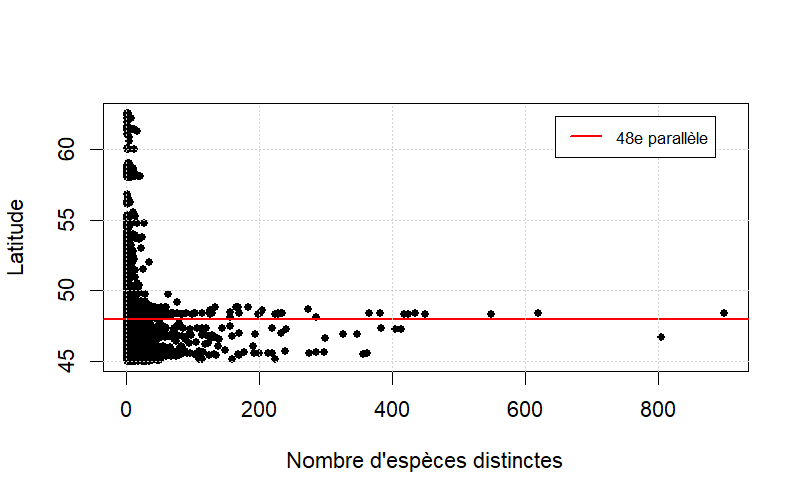
\includegraphics[width=3.5in]{lat.png}
  \caption{Richesse spécifique de lépioptères au Québec selon un gradient Nord-Sud du 45e au 65e parallèle}
\end{figure}

Pour continuer, le même processus fut suivi afin d'illustrer la
variation spécifique selon un gradient longitudinal (fig.~2). Aucune
tendance ne semble apparaître dans la variation longitudinale des
données.

\begin{figure}[H]
  \centering
  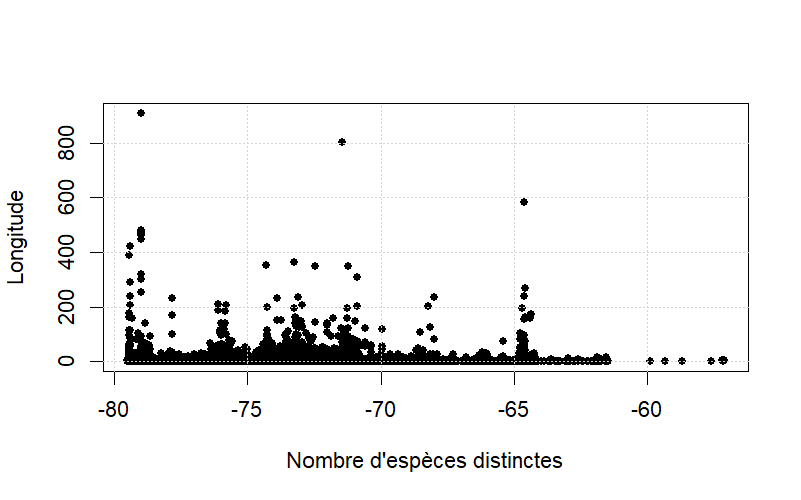
\includegraphics[width=3.5in]{lon.png}
  \caption{Richesse spécifique de lépioptères au Québec selon un gradient de longitude de -60 à -80}
\end{figure}

Par la suite, la distribution géographique des points d'observation sur
le territoire du Québec à été illustrée à l'aide de la fig.3.

\begin{figure}[H]
  \centering
  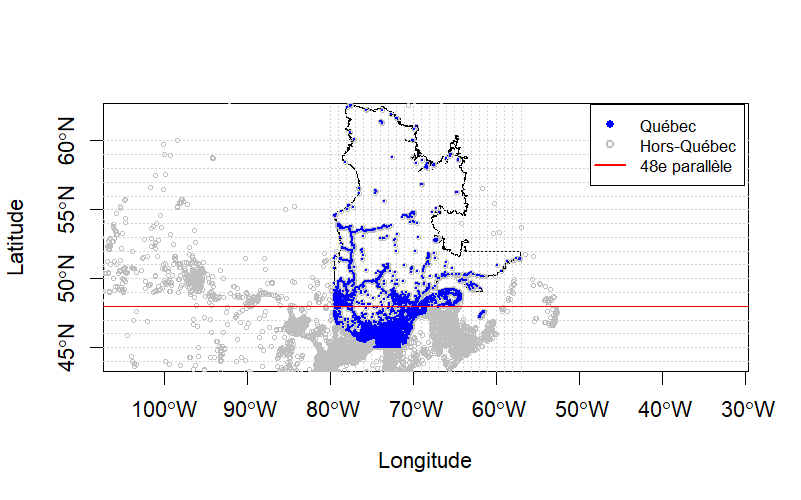
\includegraphics[width=3.5in]{quebec.png}
  \caption{Répartition géorgaphique des observations recencées de lépidoptères au Québec de 1859 à 2023}
\end{figure}

\section{Discussion}\label{discussion}

La tendance positive du nombre d'espèces selon le gradient nord-sud
pourrait s'expliquer par les différences entre les milieux climatiques
qui, eux, varient en fonction de la latitude. Tel que mentionné
précédemment, il est possible d'observer une baisse de la diversité
spécifique à partir de 48 degrés de latitude, ce qui correspond à la
transition entre la zone tempérée nordique nordique et la zone
boréale(MFFP 2022). Plus que l'on s'éloigne de la zone tempérée
nordique, plus le type des forêts passe d'érablières à des sapinières et
le climat devient plus rigoureux. En effet, vers le nord, les
précipitations diminuent, la température chute et la saison de
croissance est raccourcie (BenoÍt et al. 2002). C'est alors dans les
conditions clémentes du sud de la province que l'on y retrouve la plus
grande biodiversité de végétaux (Bégin 2022). Considérant que la
diversité des Lépidoptères est entre autres influencée par la diversité
des végétaux, la tendance semble correspondre à la littérature.

Considérant que les prédictions actuelles des changements climatiques
indiquent une tendance vers un réchauffement du climat, cela pourrait
possiblement avoir des impacts sur la répartition et la biodiversité des
espèces au Québec. En effet, si la température devient trop élevée pour
les espèces étant situées plus au sud de la province, il serait possible
que ces espèces tendent à se diriger vers le nord afin d'atteindre des
habitats plus frais(Hill et al. 2021).Cependant, même si le territoire
de la zone boréale est plus frais, il ne faut pas oublier que la
composition écosystémique n'est pas la même, demandant parfois une
adaptation rapide à une nouvelle niche écologique, ce qui constitue un
enjeu de taille pour de nombreuses espèces (Hill et al. 2021). Le
réchauffement du climat pourrait aussi engendrer une arrivée plus rapide
du printemps, causant potentiellement un décalage entre l'ouverture des
fleurs et l'activité des pollinisateurs, ce qui pourrait avoir un impact
négatif sur la valeur sélective de ces derniers(Posledovich et al.
2015). De plus, il fut d'observer que les espèces de Lépidoptères étant
adaptées aux zones arctiques et boréales sont plus sensibles aux
réchauffements climatiques que les autres espèces de papillons(Shirey et
al. 2024).

Par la suite, tel que mentionné plus haut, on peut observer qu' en
longitude, la distribution ne semble pas suivre une tendance constante.
Toutefois, il est possible d'observer qu'il y a moins d'espèces à
reporter vers l'est de la province. Cette diminution pourrait
s'expliquer par la division du territoire terrestre par de grandes
étendues d'eau à partir de ces mêmes longitudes (Figure 3).

Il faut toutefois prendre en considération qu'il existe un biais majeur
quant aux données utilisées dans cette étude, car elles proviennent en
majorité d'observations provenant de la science citoyenne. En effet, il
est difficile de savoir si les zones ayant moins d'observation découlent
d'une diversité spécifique plus faible de Lépidoptère ou si elle
correspond plutôt à une densité plus faible de population humaine, et
donc à un effort d'échantillonnage moindre. En effet, il est possible
d'observer que les régions ayant un nombre élevé d'observations semblent
correspondre avec les zones ayant une plus grande densité de population,
soit les régions du sud du Québec(Annexe 1). De plus, hors la densité de
la population, il faut aussi prendre en considération que certains
secteurs sont moins accessibles pour la prise de données. En effet,
malgré la plus faible densité de population dans la zone boréale, il est
possible d'observer sur la figure 3 des observations qui se suivent
géographiquement et qui correspondent avec la forme d'une route, telle
que pour la route 109 et son prolongement, soit la route Billy Diamond,
située au nord-ouest du Québec. Ces aspects pourraient alors expliquer,
du moins en partie, les tendances observées de la richesse spécifique
sur le territoire. Afin d'éviter ce biais et de pouvoir tirer des
conclusions justes, il faudrait alors effectuer des prises de données de
Lépidoptère de manière standardisée en utilisant le même effort
d'échantillonnage à chaque latitude et longitude. Cela permettrait alors
de tirer des conclusions plus précises quant à la répartition des
Lépidoptères.

ANNEXE 1

\begin{figure}[H]
  \centering
  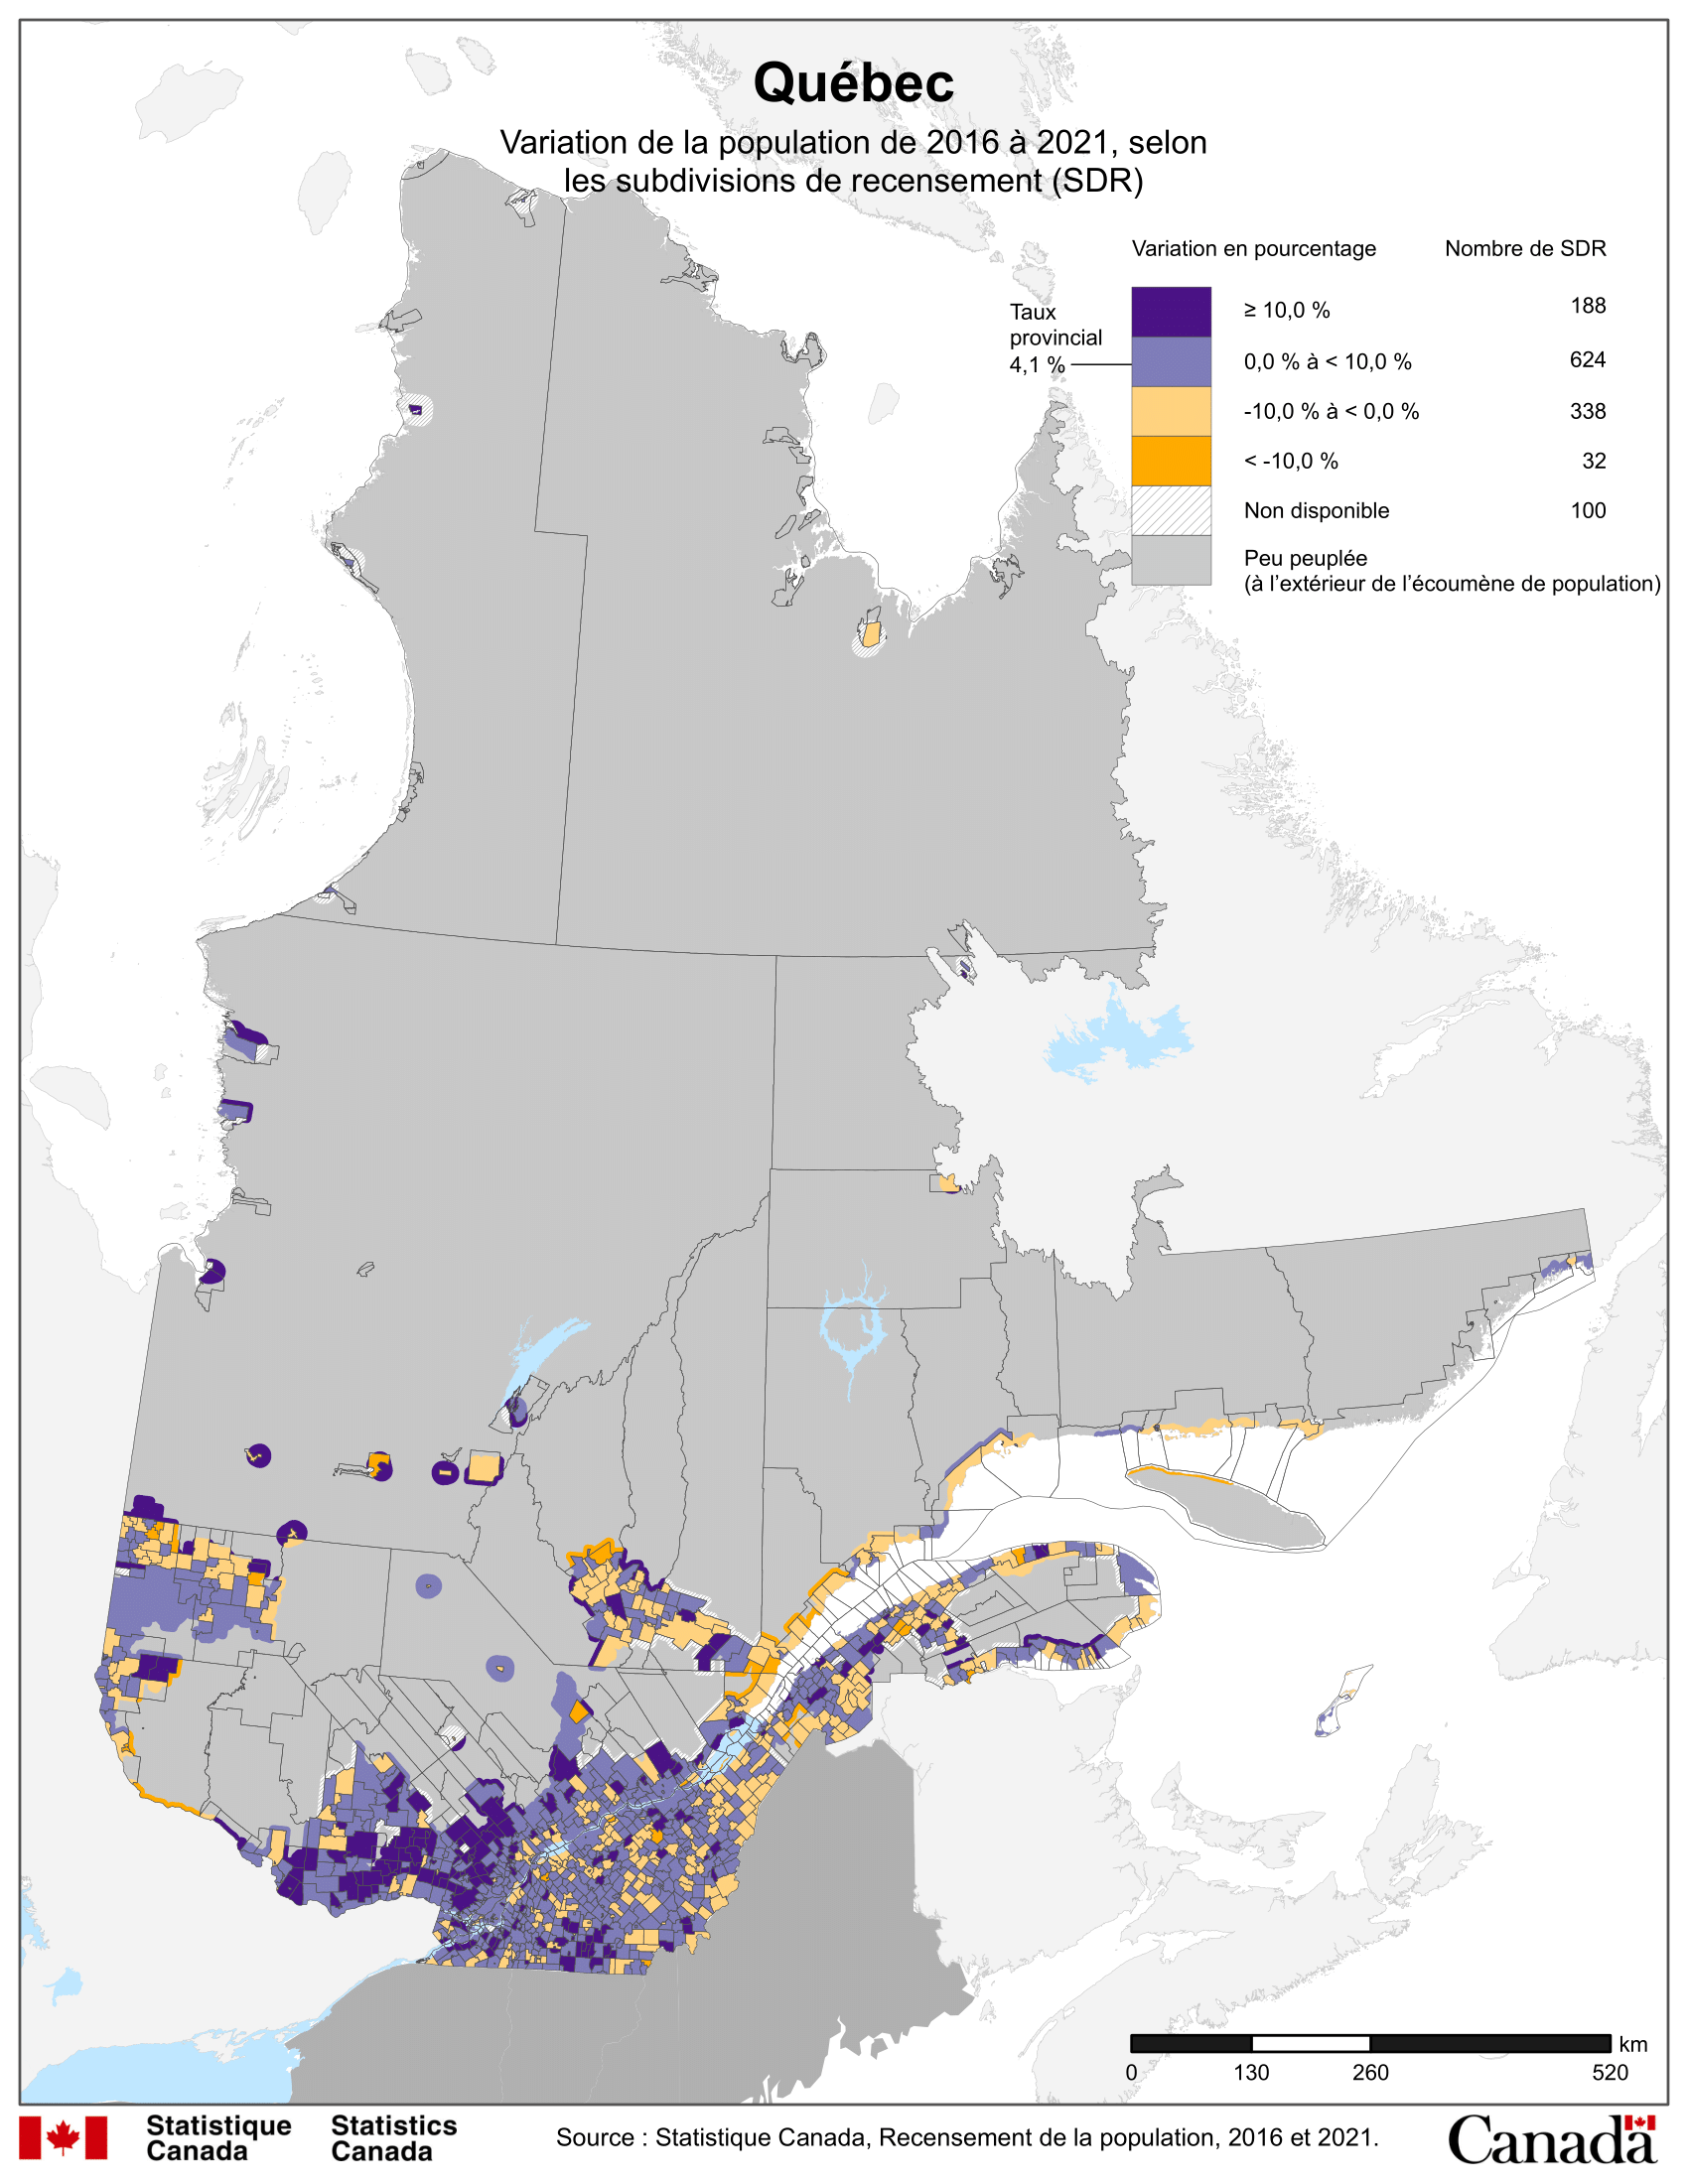
\includegraphics[width=\linewidth]{densite.png}
\end{figure}

\newpage

\section*{Réferences}\label{references}
\addcontentsline{toc}{section}{Réferences}

\protect\phantomsection\label{refs}
\begin{CSLReferences}{1}{0}
\bibitem[\citeproctext]{ref-begin_conserver_2022}
Bégin, Catherine. 2022. {``Conserver Le Sud Du {Québec}, Pourquoi Est-Ce
Si Important?''} \emph{Nature Québec}.
\url{https://naturequebec.org/conserver-le-sud-du-quebec-pourquoi-est-ce-si-important/}.

\bibitem[\citeproctext]{ref-benoit_assessing_2002}
BenoÍt, H. P., O. E. Johannsson, D. M. Warner, W. G. Sprules, and L. G.
Rudstam. 2002. {``Assessing the Impact of a Recent Predatory Invader:
{The} Population Dynamics, Vertical Distribution, and Potential Prey of
{Cercopagis} Pengoi in {Lake} {Ontario}.''} \emph{Limnology and
Oceanography} 47 (3): 626--35.
\url{https://doi.org/10.4319/lo.2002.47.3.0626}.

\bibitem[\citeproctext]{ref-edwards_rapid_2025-1}
Edwards, Collin B., Elise F. Zipkin, Erica H. Henry, Nick M. Haddad,
Matthew L. Forister, Kevin J. Burls, Steven P. Campbell, et al. 2025.
{``Rapid Butterfly Declines Across the {United} {States} During the 21st
Century.''} \emph{Science} 387 (6738): 1090--94.
\url{https://doi.org/10.1126/science.adp4671}.

\bibitem[\citeproctext]{ref-hill_climate_2021}
Hill, Geena M., Akito Y. Kawahara, Jaret C. Daniels, Craig C. Bateman,
and Brett R. Scheffers. 2021. {``Climate Change Effects on Animal
Ecology: Butterflies and Moths as a Case Study.''} \emph{Biological
Reviews} 96 (5): 2113--26. \url{https://doi.org/10.1111/brv.12746}.

\bibitem[\citeproctext]{ref-mcelwee_climate_2021}
McElwee, Pamela. 2021. {``Climate {Change} and {Biodiversity} {Loss}:
{Two} {Sides} of the {Same} {Coin}.''} \emph{Current History} 120 (829):
295--300. \url{https://doi.org/10.1525/curh.2021.120.829.295}.

\bibitem[\citeproctext]{ref-mffp_zones_2022}
MFFP. 2022. {``Zones de Végétation Et Domaines Bioclimatiques Du
{Québec}.''}

\bibitem[\citeproctext]{ref-posledovich_developmental_2015}
Posledovich, Diana, Tenna Toftegaard, Christer Wiklund, Johan Ehrlén,
and Karl Gotthard. 2015. {``The Developmental Race Between Maturing Host
Plants and Their Butterfly Herbivore -- the Influence of Phenological
Matching and Temperature.''} Edited by Jonathan Newman. \emph{Journal of
Animal Ecology} 84 (6): 1690--99.
\url{https://doi.org/10.1111/1365-2656.12417}.

\bibitem[\citeproctext]{ref-shirey_rising_2024}
Shirey, Vaughn, Naresh Neupane, Robert Guralnick, and Leslie Ries. 2024.
{``Rising Minimum Temperatures Contribute to 50 Years of Occupancy
Decline Among Cold‐adapted {Arctic} and Boreal Butterflies in {North}
{America}.''} \emph{Global Change Biology} 30 (2): e17205.
\url{https://doi.org/10.1111/gcb.17205}.

\end{CSLReferences}

\end{document}

